\chapter{Evaluation} \label{chap:eval}

Until now, we showed various possibilities of constructing a classification model.
In this chapter, we describe how to compare their performance.
We cannot mathematically prove that a model is a correct estimation of what we are trying to classify.
This is because we do not know the actual real distribution of data and can only estimate it.
Therefore, we use statistical methods on a testing set.

We cannot validate a model based on how well it fits our training data.
Doing that would yield over-optimistic results, because our model is optimized for it.
Also, it would not give us any idea how well the classifier performs on data it has not seen during the training phase.
Hence, we need to have a special testing set used only for evaluating.
Finally, we introduce different metrics for expressing various properties of a model.

\section{Overfitting}

The described problem of over-optimistic results is called overfitting.
{\bf Overfitting} (sometimes referred to as {\bf bias}) means
that our model is able to predict instances it has been trained on a lot better than new instances. 
We say that a model does not generalise well.
This happens when an algorithm learns to recognise idiosyncrasies of the training set,
rather than to understand the underlying logic.
These idiosyncrasies can appear by incomplete data, noise introduced during obtaining the data or
irrelevant information leading to incorrect labelling.

Instead of having simple and robust rules to describe data,
we have many random rules that work for only small subsets of data.
Our objective describes a phenomenon known as {\it Occam's razor}.
As stated in \citet{sammut2011encyclopedia}, it is often interpreted as
``a less complicated solution being preferred over a more complicated one''.
The less complicated solution is less likely to suffer from overfitting,
because there is simply not enough space to include all various idiosyncrasies.
An example of such a process can be a {\bf Decision Tree}.
If we have two trees with comparable performance,
the one with less nodes is more likely to generalise better.
\citet{TanBachKum08} describe this in more detail in chapter 4.

\section{Partitioning Data}

Usually, we do not get data divided into training and testing sets.
Even though it gives us more flexibility, it also introduces a new challenge how to obtain the two sets.
We will present two methods of diving data into these sets.
First, a very simple holdout method.
Second, k-fold cross validation which builds on top of holdout.

\subsection{Holdout Method}

The simplest approach, called \textbf{holdout}, is to randomly divide data into two sets,
such that their sizes will be in a specific ratio.
The exact ratio is at the discretion of further analysis and it needs to balance two crucial requirements.

First, not enough data may lead to lower performance, so we want to train the model on as much data as we possibly can.
Second, if we use too much data for training, the performance evaluation will be less reliable.
Statistically speaking, it will have a wider confidence interval.

As \citet{TanBachKum08} note, another problem is with obtaining an independent set.
The training set can be chosen in such a way that it contains biased data.
We also should be aware of the fact that training and testing sets are no longer independent,
because the entire dataset is split between the two.
Because of this reason, particular choice of one set directly influences the properties of the other.

An example of this dependency is the distribution of labels.
Suppose there are 80\% positive and 20\% negative instances.
If we choose the training set such that 90\% instances are positive,
there will be less than 80\% positive instances in the testing set.

A way of overcoming this problem is \textit{stratification}.
\citet{sammut2011encyclopedia} define it as a way of keeping the class
distribution as close as possible across all sets.
More on this can be found in  \citet{TanBachKum08} in chapter Sampling.


\subsection{Cross-Validation}

To address some of the issues listed above, {\bf Cross-Validation} has been introduced.
The underlying idea is that each instance is used the same number of times for training 
and exactly once for testing.
We split the dataset into~$k$~equally-sized subsets.
For each subset, we train our algorithm on all subsets but the one chosen 
and the one will be used as a testing set.
This approach is called {\bf k-fold cross-validation} for~$k$~subsets.
The variable~$k$~is chosen arbitrarily.

Special case for~$k=N$ where~$N$~is the number of instances is called {\bf leave-one-out}
and has the advantage of 
utilizing as much data for training as we can.
However, it is computationally expensive and
we therefore generally choose a lower value of~$k$~for practical reasons.

Thorough description of cross-validation along with other partitioning schemes
can be found in \citet{arlot2010}.

In this thesis, we compute evaluation metrics for each pair of training and testing sets separately
and report their average along with minimal and maximal value and standard deviation.


\section{Evaluation Metrics}

When we have our training and testing sets, we can train our classifier.
Subsequently, we predict labels of instances in the testing set with our newly
built classifier.
To say how well the classifier performs, we need to express how well the predicted
labels fit the actual labels.
For doing this we will introduce several {\bf evaluation metrics}.

Let us have a binary classification problem and a classifier we want to evaluate.
For evaluation, we always have to decide which label we will evaluate it on.
In our case we will choose ``useful''.
All instances that our classifier predicted as this label are then {\bf positive} 
and the rest are {\bf negative}.
Both categories are further divided into true and false;
true being instances that our classifier predicted correctly and false, incorrectly.
Together we have four categories:
true positive, false positive, true negative and false negative.
For clarity we can arrange these four categories into the so-called {\bf confusion matrix} 
as shown in \Cref{tab:confmatrix}.
Each cell represents the number of instances from one of the categories.
The columns correspond to instances where the predicted label is the chosen one (\textit{yes}) and the rest (\textit{no}).
Analogously, rows correspond to instances with the chosen label (\textit{yes}) and the rest (\textit{no}).
Diagonal {\it TP} and {\it TN} represents all instances that have been classified correctly.
The other diagonal represents all misclassified instances.



%then matrix~$A$~of the dimensions 2x2 is a {\bf confusion matrix} if and only if~$A_{1,1}$~and~$A_{1,2}$~are the numbers of correctly and incorrectly classified positive instances, respectively. $A_{2,1}$ and~$A_{2,2}$~are then analogically correctly and incorrectly classified negative instances.

\begin{table}[h!]
\center
\begin{tabular}{ll|c|c|}
\cline{3-4}
& & \multicolumn{2}{c|}{predicted label} \\
\cline{3-4}
& & \hbox to 1cm{\hfil yes\hfil} & \hbox to 1cm{\hfil no\hfil} \\
\hline
\multicolumn{1}{|l|}{actual}& yes & TP & FN\\
\cline{2-4}
\multicolumn{1}{|l|}{label}						   & no & FP & TN \\
\hline

\end{tabular}
	\caption{Confusion Matrix}\label{tab:confmatrix}
\end{table}

In the example below, we have 10 and 11 instances classified correctly. 
They are true positives and true negatives respectively.
There are 5 instances classified as not-useful, but actually being useful.
These are false negatives.
The last cell represents 2 not-useful instances classified as useful --- these are false positives.

\begin{table}[h!]
\center
\begin{tabular}{ll|r|r|}
\cline{3-4}
& & \multicolumn{2}{l|}{predicted label} \\
\cline{3-4}
& & \hbox to 1.2cm{\hfill useful\hfil} & \hbox to 1.2cm{\hfill not\hfil} \\
\hline
\multicolumn{1}{|l|}{actual}& useful & 10 & 5\\
\cline{2-4}
\multicolumn{1}{|l|}{label}						   & not & 2 & 11 \\

\hline

\end{tabular}
	\caption{An Example of Confusion Matrix}\label{tab:confmatrix_ex}
\end{table}


The most straightforward metrics are accuracy and error rate.
{\bf Accuracy} is the ratio of correctly classified instances and {\bf error rate} incorrectly.
In the confusion matrix it is:

\newcommand\TP{\mathit{TP}}  % ty makra nejsou nutna, ale setri praci; mathit je treba, aby to melo spravne mezery
\newcommand\TN{\mathit{TN}}
\newcommand\FP{\mathit{FP}}
\newcommand\FN{\mathit{FN}}
\newcommand\ALL{\mathit{All}}
\begin{equation}
\mathit{accuracy} = \frac{\TP + \TN}{\TP + \TN + \FP + \FN}
\end{equation}

A complementary measure to accuracy is error rate:
\begin{equation}
\mathit{error~rate} = 1 - \mathit{accuracy}
\end{equation}
or equivalently
\begin{equation}
\mathit{error~rate} = \frac{\FP + \FN}{\TP + \TN + \FP + \FN}
\end{equation}

In our mock example accuracy is~$21/28$ and error rate~$7/28$.

More commonly used metrics for their better properties are precision, recall and f-measure.
{\bf Precision} is the ratio of correctly classified instances out of those classified as positive.
It expresses our confidence on how likely an instance is positive when we classify it so.

\begin{equation}
\mathit{precision} = \frac{\TP}{\TP + \FP}
\end{equation}

{\bf Recall} is the ratio of how many instances were classified as positive
outside of those that are truly positive.
It expresses our confidence on how many truly positive instances we can correctly identify.

\begin{equation}
\mathit{recall} = \frac{\TP}{\TP + \FN}
\end{equation}

In our toy example precision and recall are~$10/12$~and~$10/15$~respectively.

To combine recall and precision, {\bf f-measure} is commonly used.
It is the harmonic average of the two and expresses the combination of both properties.

\begin{equation}
	\mathit{F\mbox{-}measure} = 2 \times \frac{\mathit{precision}\times \mathit{recall}}{\mathit{precision} + \mathit{recall}}
\end{equation}


More thorough description of evaluation can be found in \citet{TanBachKum08}.


\subsection{Learning Curves}\label{sec:lcurves}

As \citet{sammut2011encyclopedia} describe it,
\textbf{learning curves} is a way of representing how well the model  generalizes.
It is a way of finding reasons why our model performs poorly.

In a general machine learning setting, learning curves are a visualization of a function
of the model performance relative to the size of the training set.
Usually, this function is plotted for both training and testing set.
This a bit counter intuitive approach shows how well the model
actually fits the training data and how well it is able to predict unseen instances.
As well as the actual different between seen and unseen data.

Detailed description can be found in \citet{cortes1994learning}.
An example taken from the article can be see in \Cref{fig:l_c_ex}.
It shows a typical classifier.
Training error is lower than testing, but asymptotically they reach the same value.
By looking much close the curves get, we may estimate how much data is needed
to prevent overfitting.


\begin{figure}[ht]\centering
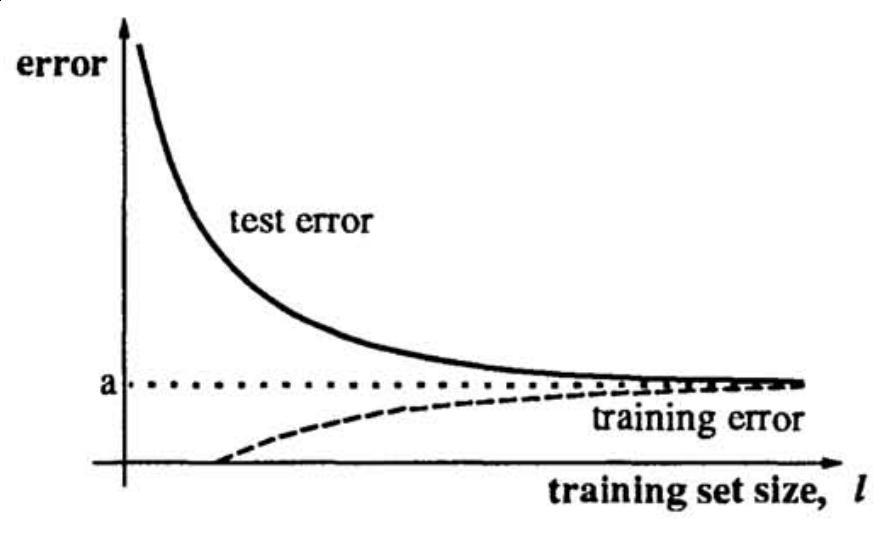
\includegraphics[width=100mm]{../img/learning_curves_example.png}
\caption{Example of learning curves for a classifier}
This example has been taken from \citet{cortes1994learning}.
\label{fig:l_c_ex}
\end{figure}


If the testing error is significantly higher than training error,
we may say by looking at the graph, whether
the model suffers from overfitting.
In that case, the curves would not asymptotically be the same value.
If, on the other hand, both curves showed high error,
the model would be unlikely to be good in general.


In this chapter, we discussed what properties of classification are desirable
and outlined how to use data for evaluating the performance.
At the end, we introduced evaluation metrics.
